\documentclass[10 pt,Helvetica, french]{beamer}
% option compress pour réduire la taille des bars
\mode<presentation>
%[compress,hideallsubsections,width=<0.5cm>]
%\usetheme{Darmstadt}
%\usetheme{Malmoe}
%\usetheme{Warsaw}
%\useoutertheme{split}
%\usecolortheme{whale}

%\usepackage[dark]{beamerthemesidebar}
%\usepackage{beamerthemeshadow}
%\usepackage{beamerthemesplit}
%\usepackage{beamerthemebars}
%\usepackage{beamerthemeclassic}
\newcommand{\spac}{\rule[0mm]{0mm}{2mm}}
\usepackage{pgf,pgfarrows,pgfnodes,pgfautomata,pgfheaps,pgfshade}
\usepackage{amsmath,amssymb}
\usepackage[english]{babel}
\usepackage{epic,eepic,bez123}
\usepackage{ bbold }
\usepackage{ upgreek }
\usepackage{eurosym}
\usepackage{color}
%\usepackage[T1]{fontenc}
%\usepackage[ansinew]{inputenc}
%\usepackage[latin1]{inputenc}
%\usepackage{babel,varioref}

%\usetheme{Luebeck}%(encadrements rectangulaires)
%\usetheme{Madrid}%(pas de plan au-dessus)
%\usetheme{Berkeley}%(colonne à gauche)
%\usetheme{Warsaw}%(plan détaillé en haut, utilise la navigation)
%\usetheme{Dresden}%(encadrements rectangulaires)
%\usetheme{Frankfurt}%(pas de paln détaillé en haut)
%\usetheme{Marburg}%(colonne à droite)
%\usetheme{Berlin}%(encadrements rectangulaires)
%\usetheme{Montpellier}

%\usecolortheme{crane}
%\usecolortheme{seahorse}
%\usecolortheme{green}
%\usecolortheme{beetle}
%\usecolortheme{default}
%\usecolortheme{rose}
%\usecolortheme{Berkeley}(inconnu)

%\useoutertheme{smoothtree}
%\useoutertheme{split}
%\usecolortheme{whale}

\setbeamercovered{transparent}
\newtheorem{defi}{Definition}
\newtheorem{theo}{Theorem}
\newtheorem{prop}{Proposition}
\newtheorem{property}{Property}
\newtheorem{coro}{Corollary}
\newtheorem{propannex}{Proposition}
\newtheorem{objective}{Objective}
\newtheorem{res}{Results}


\setbeamertemplate{footline}[text line]{  }
%\setbeamertemplate{footline}[page number]{ }

\newcounter{countAnnexA}
\setcounter{countAnnexA}{0}
\renewcommand{\propannex}{\addtocounter{countAnnexA}{1}
\noindent \large \textbf{Proposition \thesection.\thecountAnnexA}
\normalsize}

\newcommand{\beginbackup}{
   \newcounter{framenumbervorappendix}
   \setcounter{framenumbervorappendix}{\value{framenumber}}
}
\newcommand{\backupend}{
   \addtocounter{framenumbervorappendix}{-\value{framenumber}}
   \addtocounter{framenumber}{\value{framenumbervorappendix}}
}

%\colorlet{orange}{red!70!yellow}% mes petites couleurs que j'aime bien
%\colorlet{mauve}{blue!70!red} \colorlet{brouge}{red!70!blue}
\addtobeamertemplate{footline}{\insertframenumber/\inserttotalframenumber}


\date[September 2017]{DEGIT Conference, September 2017}
\title[Trade Costs Black Box]{Beyond the Iceberg Hypothesis: \\Opening the Black Box of Transport Costs}
\author[Daudin et al.]{Guillaume Daudin\\
{\footnotesize Universit\'{e} Paris-Dauphine, PSL \& OFCE }\\ \smallskip
J\'{e}rome H\'{e}ricourt \\
{\footnotesize Universit\'{e} de Lille I \& CEPII }\\  \smallskip
Lise Patureau \\
{\footnotesize  Universit\'{e} Paris-Dauphine, PSL}}


\setcounter{framenumber}{-1}
\begin{document}
\begin{frame}[plain]
\titlepage
\end{frame}


\begin{frame}
\frametitle{Motivation}
\begin{itemize}
\item Trade costs have a central role in international economic analysis \vspace{0.1cm}
\begin{itemize}
\item[-] Declining over the second half of the 20$^{th}$ century (Jacks et al., 2008, Novy, 2013) \vspace{0.1cm}
\item[-] But still significant: Average international trade costs = a 74\% markup over production costs (Anderson \& Van Wincoop, 2004)
\end{itemize}
\item What exactly are ``trade costs''?  \vspace{0.1cm}
\begin{itemize}
\item[-] Transaction costs, policy costs, time costs, and transport costs \textit{per se}
\end{itemize}
\item Transport costs are a sizeable share of international trade costs \vspace{0.1cm}
\begin{itemize}
\item[-]  Amount to $\simeq 30\%$ of international trade costs  $\Leftrightarrow$ A 21\% markup over production costs  \vspace{0.1cm}
%\item[-] Elasticity of trade wrt freight costs = -3 (Behar \& Venables, 2011) \vspace{0.1cm}
\end{itemize}
\item[$\Rightarrow$] If much trade policy barriers have been removed, the transport cost component of trade costs remains sizeable \vspace{0.1cm}
\end{itemize}
\textbf{The paper: On international transport costs}

\end{frame}

\begin{frame}
\frametitle{Motivation (cont')}
\begin{itemize}
\item Standard modeling of trade costs: As an ad-valorem tax-equivalent \vspace{0.1cm}
\begin{itemize}
\item[-] As a constant percentage of the producer price per unit traded \vspace{0.1cm}
\item[$\Leftrightarrow$] Part of the ``iceberg cost'' hypothesis (Samuelson, 1954) \vspace{0.1cm}
\begin{itemize}
\item[$\ast$] With $p$ the import price, $\widetilde{p}$ the export price, $q$ the quantity traded and $\tau >1$ the trade cost \vspace{0.1cm}
\item[$\Rightarrow$] Multiplicative costs:     \footnotesize $pq = \tau \widetilde{p}q$
\normalsize
\end{itemize}
\end{itemize}
\item Yet... A debated question \vspace{0.1cm}
\item Would not trade costs rather exhibit an additive structure ?  \vspace{0.1cm} \vspace{0.1cm}
\begin{itemize}
\item[-] Why would it be more costly to transport from Milan to Paris, a pair of Italian shoes at price \euro 300 than a pair of Italian shoes at price \euro 50? \vspace{0.1cm}
\item[-] Pricing shipping often includes an additive component \vspace{0.1cm}
\begin{itemize}
\item[$\ast$] UPS: A \$125 fee charged for a 2 pound package from Oslo to NYC (Irrarazabal et al., 2015) \vspace{0.1cm}
%\item[$\ast$] Some trade policy instruments as well (quota license price) \vspace{0.1cm}
\item[$\Rightarrow$] Additive costs: \footnotesize $pq = (t+\widetilde{p})q  $
\end{itemize}
\end{itemize}
\end{itemize}
\end{frame}


\begin{frame}
\begin{itemize}
\item Recent empirical evidence in support of the additive structure of trade costs \vspace{0.1cm}
\begin{itemize}
\item[-] Irrarazabal et al. (2015), Hummels \& Skiba (2004), Martin (2012)  \vspace{0.2cm}
\end{itemize}
\item The structure (additive vs iceberg) of transport costs is not anecdotal \vspace{0.1cm}
\begin{itemize}
\item[-] Additive costs play an important role in shaping the pattern of trade flows (Alchian \& Allen, 1964) \vspace{0.1cm}
\item[-] Strong normative implications, notably w.r.t. the welfare gains of trade liberalization (Sorensen, 2014)\vspace{0.1cm}

\end{itemize}
\item[$\Rightarrow$] Transport costs are likely to display an additive component, but precisely... by how much? \vspace{0.2cm}
\end{itemize}
\textbf{One objective of the paper: Provide an answer to this question}

\end{frame}


\begin{frame}
\frametitle{Our paper in one question (and 3 answers)}

\begin{itemize}
\item  \textbf{Do additive transport costs matter?} \vspace{0.1cm}
\begin{itemize}
\item[-] Provide an empirical decomposition of the structure of transport costs \vspace{0.1cm}
\item[-] Using the US imports database over 1974-2013 (air/vessel)\vspace{0.2cm}
\end{itemize}
\item[$\Rightarrow$] \textbf{Yes, they do} \vspace{0.1cm}

\item[(1)] \textbf{In terms of size}: Additive costs are sizeable \vspace{0.1cm}
\begin{itemize}
%\footnotesize{
\item[-] Additive cost: 1.8\% and 2.9\% of the export price, in air / vessel \vspace{0.1cm}
%\item[-] Iceberg cost: 2.5\% of the export price in air, and 3.2\% in vessel (mean value over 1974-2013) \vspace{0.1cm}
\item[-] Roughly 50\% of the overall transport costs \vspace{0.1cm}

%}
\end{itemize}
\item[(2)] \textbf{In terms of quality of fit}: With the additive component included, \vspace{0.1cm}
\begin{itemize}
%\footnotesize{
\item[-] The estimated iceberg component is reduced by a factor of 2 \vspace{0.1cm}
\item[-] A substantially better ``goodness-of-fit'' %}
%}
\end{itemize}
\end{itemize}
\end{frame}

\begin{frame}
\begin{itemize}
\item[(3)] \textbf{In accounting for the time trend of transport costs} \vspace{0.2cm}
\begin{itemize}
\item[-] The modelling of the additive component of transport costs is key \vspace{0.1cm}
\item[-] Because it changes the result of excluding the trade composition effects when characterizing the time trend \vspace{0.1cm}
\begin{itemize}
\item[$\ast$] The decrease in TC over time is mostly attributable to the decrease in the ``pure'' transport costs,  \vspace{0.1cm}
\item[$\ast$] Rather than to trade composition effects  \vspace{0.1cm}
\end{itemize}
\item[-] A result in sharp contrast with Hummels (2007) \vspace{0.2cm}
\end{itemize}
\end{itemize}
\textbf{All our results: Provide new quantitative evidence about the importance of the additive component in international transport costs}

\end{frame}


\begin{frame}
\frametitle{Plan of the talk}
\begin{itemize}
\item Data Sources  \vspace{0.2cm}
\item Empirical Methodology \vspace{0.2cm}
\item Results \vspace{0.2cm}
\item Conclusion
\end{itemize}
\end{frame}


\begin{frame} [label=slide_data]
\frametitle{Data sources}
\begin{itemize}
\item Our measure of international transport costs: The difference between the ``export'' price and the ``import'' price of US imports\vspace{0.1cm}
\item Database: US Imports of Merchandise database \vspace{0.1cm}
\begin{itemize}
\item[-] The export (fas) price, $\widetilde{p}$: the price for one kg of merchandise at the country export point \vspace{0.1cm}
\item[-] The import (cif) price, $p$: the price for one kg of merchandise at the entry in the US \vspace{0.1cm}
\item[-] Yearly basis, from 1974 to 2013, SITC 5-digit classification level, by transport mode (air or vessel) \vspace{0.1cm}
%(Could go up to HS-10 with recent data)\vspace{0.1cm}
\end{itemize}
\item[$\Rightarrow$] Our dependent variable: Based on the ratio $p/\widetilde{p}$ \vspace{0.1cm}
\item The RHS is at the 3-digit classification level  \vspace{0.1cm}
\begin{itemize}
\item[-] Estimation at the 4-digit level on some selected years as robustness \vspace{0.1cm}
\item[-] Approximatively 200 sectors (3 digits), from around 200 countries  \vspace{0.1cm}
\begin{itemize}
\item[$\ast$] Around 600-700 sectors at the 4-digit level
\end{itemize}
\end{itemize}
\end{itemize}
\end{frame}

\begin{frame}
\frametitle{More on our database}
\begin{itemize}
\item Implications (and limitations) \vspace{0.1cm}
\begin{itemize}
\item[-] Only cover international transport costs \vspace{0.1cm}
\item[-] Among transport costs, insurance + handling + quantitative freight costs (e.g. not those related to the time value of goods) \vspace{0.1cm}
%\item[$\Leftrightarrow$] Among the 21\% markup from AVW, $\simeq$ 11\% for freight costs (the remaining 9\% for time costs). But ``rough'' estimate. Precisely?  \vspace{0.1cm}
\end{itemize}
\item A rich database to exploit \vspace{0.1cm}
\begin{itemize}
\item[-] US imports, long time period: Broad view of international trade flows \vspace{0.1cm}
\item[-] A reliable database, already used by Hummels (2007), but on a shorter length of time \vspace{0.1cm}
\item[-] Have both the import and the export prices  \vspace{0.1cm}
\item[$\Rightarrow$] Allows the estimate the levels of both the ad-valorem and the additive transport costs  \vspace{0.1cm}
\begin{itemize}
\item[$\neq$] Irarrazabal et al. (2015)
\end{itemize}
\end{itemize}
\end{itemize}
\end{frame}

\begin{frame}
\frametitle{Empirical specification (1)}
\textbf{The equation at the root of the estimation}
\begin{itemize}
\item Relate the import price $p$ to the export price $\widetilde{p}$ given both additive (per-kg) costs $t$ and ad-valorem costs $\tau$:
$$p = \tau \widetilde{p} + t, \qquad \text{with}\quad \tau \geq 1,\quad t \geq 0$$
\item From country $i$, for a product $k$ (at the $k=$ 5-digit classification level, and for a given transport mode)   \vspace{0.1cm}
\item Rewrite to get:
\begin{equation}
\frac{p_{ik}}{\widetilde{p}_{ik}} -1 = \tau_{ik} -1 +\frac{t_{ik}}{ \widetilde{p}_{ik}} \label{eq:basis_equation}
\end{equation}
\item[$\Rightarrow$] For each year over 1974-2013\vspace{0.1cm}
\begin{itemize}
\item[-] The equation is also mode (air or vessel) - specific
\end{itemize}
\end{itemize}
\end{frame}

\begin{frame}[label = slide_empirical_strategy]
\frametitle{Empirical specification (2)}
\textbf{Obtain the estimated equation}
\begin{itemize}
\item Make some simplifying assumptions \hyperlink{app_empirical_strategy}{\beamergotobutton{More details}}  \vspace{0.1cm}
\begin{itemize}
\item[-] About the specification of both additive and multiplicative costs  \vspace{0.1cm}
\begin{itemize}
\item[$\ast$] Separability between the product and the country dimensions (as Irarrazabal et al., 2015)   \vspace{0.1cm}
\item[$\ast$] All products $k$ in a 3-digit sector ($s$) share the same structure of costs  \vspace{0.1cm}
\end{itemize}
\item[-] About the specification of the error term \vspace{0.1cm}
\end{itemize}
\item Taking logs, we finally estimate the following equation:
\footnotesize
\begin{equation*}
\ln\left(\frac{p_{ik}}{\widetilde{p}_{ik}}-1 \right)= \ln \left(\tau_{i} \times \tau_{s(k)}+\frac{t_{i} + t_{s(k)}}{\widetilde{p}_{ik}}-1 \right) + \epsilon_{ik}
\end{equation*}

\begin{itemize}
\footnotesize
\item[-] With $\epsilon_{ik}$ following a normal law centered on 0  \vspace{0.1cm}
\item[-] $\tau_i$, $\tau_{s(k)}$, $t_i$, $t_{s(k)}$ are the parameters (i.e. fixed effects) to be estimated
\end{itemize}
\normalsize
\item A non-linear equation (due to the additive costs)  
\item[$\Rightarrow$] Estimation using non-linear squares 
\end{itemize}
\end{frame}

\begin{frame}
\frametitle{Empirical specification (3)}
\textbf{How to characterize the importance of additive costs relatively to ad-valorem?} \vspace{0.1cm}
\begin{itemize}
\item Estimate Equation (\ref{eq:est_equation}) constraining $t=0$ \vspace{0.1cm}
\item[$\Rightarrow$] Estimate \textit{two} models\vspace{0.1cm}
%\begin{itemize}
\item[(A)] With additive costs excluded (only ad-valorem costs):
\footnotesize
\begin{equation}
\ln\left(\frac{p_{ik}}{\widetilde{p}_{ik}}-1 \right)= \ln \left(\tau_{i} \times \tau_{s(k)}-1 \right) + \epsilon^{ice}_{ik} \label{eq:model_nlI}
\end{equation}
\normalsize
\item[(B)] With additive costs included:
\footnotesize
\begin{equation}
\ln\left(\frac{p_{ik}}{\widetilde{p}_{ik}}-1 \right)= \ln \left(\tau_{i} \times \tau_{s(k)}+\frac{t_{i} + t_{s(k)}}{\widetilde{p}_{ik}}-1 \right) + \epsilon_{ik} \label{eq:est_equation}
\end{equation}
\normalsize
\begin{itemize}
\item[$\ast$] Under Model (B), $\simeq$ 800 fixed effects to estimate  \vspace{0.1cm}
\item[$\ast$] For each year over 1974-2013, by transport mode (air/vessel)
%\end{itemize}
\end{itemize}
\end{itemize}
\end{frame}


\begin{frame}
\begin{itemize}
\item After running the estimates, we re-built: \vspace{0.1cm}
\begin{itemize}
\item[(A)] With only iceberg costs (from Equation (\ref{eq:model_nlI})):
$$\widehat{\tau}^{ice}_{is} = \widehat{\tau_{i}} \times \widehat{\tau_{s}}$$
\item[(B)] With additive costs included (from Equation (\ref{eq:est_equation})):
$$\widehat{\tau}^{adv}_{is} = \widehat{\tau_{i}} \times \widehat{\tau_{s}}, \qquad \widehat{t}_{is} = \widehat{t}_{i} + \widehat{t}_{s}$$
\end{itemize}
\item  Taking the weighted average over the sector-country dimension, we finally get, by year and transport mode: \vspace{0.1cm}
\begin{itemize}
\item[-] With only iceberg costs: $\widehat{\tau}^{ice}$ \vspace{0.1cm}
\item[-] When additive costs are included: $\widehat{\tau}^{adv}$, $\widehat{t}$  

\end{itemize}
\end{itemize}
\end{frame}

\begin{frame}
\frametitle{Question, and answers}
\begin{itemize}
\item Do additive costs matter? \vspace{0.5cm}
\item How we answer (yes) to this question
\end{itemize}
\end{frame}

\begin{frame}[label=slide_result1]
\frametitle{Result 1: Size of additive transport costs \hyperlink{app_result1}{\beamergotobutton{More on this}} }
\begin{itemize}
\item Estimate the values of both the ad-valorem and the additive components \vspace{0.1cm}
\begin{itemize}
\item[-] \footnotesize{Average values over 1974-2013, in percent of the export price \hyperlink{app_results_summary}{\beamergotobutton{More}}  } \vspace{0.1cm}
\end{itemize}
\end{itemize}
\begin{table}[htbp]
  \centering
  \scriptsize{
  %\caption{Transport costs estimates: Summary \label{tab:summary_results}}
 \begin{center}
    \begin{tabular}{l|cc|cc}
      \hline \hline
    \multicolumn{5}{c}{Mean value over 1974-2013}   \\
    \# digit & \multicolumn{2}{c}{3 digits} & \multicolumn{2}{c}{4 digits ($^\ast$)} \\ \hline
    Mode  & Vessel & Air ($^{\ast \ast}$) & Vessel & Air \\ \hline
    \multicolumn{5}{l}{\textbf{Model (A) - With only Ad-Valorem Transport Costs} ($\widehat{\tau}^{ice}$, in \%)}  \\ \hline
    Mean  & \textcolor{red}{5.8} & \textcolor{red}{5.1} & 6.0 & 4.9 \\
    Median & 5.1 & 4.2 & 5.2 & 3.7 \\ \hline
    %Std   & 0.032 & 0.042 & 0.036 & 0.045 \\
    %Min. value & 1.003 & 1.001 & 1.003 & 1.000 \\
    %Max. value & 1.304 & 1.685 & 1.408 & 2.051 \\ \hline
    \multicolumn{5}{l}{\textbf{Model (B) - With Additive \& Ad-Valorem Transport Costs} } \\ \hline
   \textit{Ad-valorem term ($\widehat{\tau}^{adv}$, in \%)} & & & & \\ \hline
    Mean  & \textcolor{red}{3.2} & \textcolor{red}{2.5} & 3.3 & 2.4 \\
    Median & 2.8 & 1.8 & 2.8 & 1.6 \\ \hline
    %Std   & 0.023 & 0.023 & 0.025 & 0.026 \\
    %Min. value & 1.001 & 1.000 & 1.000 & 1.000 \\
    %Max. value & 1.227 & 1.474 & 1.264 & 1.537 \\ \hline
    \textit{Additive term ($\widehat{t}/\widetilde{p}$, in \%)}& & & &   \\ \hline
    Mean  & \textcolor{blue}{2.9} & \textcolor{blue}{1.8} & 2.8 & 1.9 \\
    Median & 1.9 & 0.7 & 1.7 & 0.8 \\ \hline
    %Std   & 0.041 & 0.034 & 0.039 & 0.034 \\
    %Min. value & 0.000 & 0.000 & 0.000 & 0.000 \\
    %Max. value & 2.941 & 13.303 & 3.197 & 11.440 \\ \hline
    \multicolumn{5}{l}{\textbf{Data} ($p/\widetilde{p}$, \textit{in \%})} \\ \hline
        Mean & 5.3 & 5.0& 5.6&3.9 \\
        Median & 4.3 & 2.0 & 4.4& 1.9 \\ \hline
        \# obs. & 29279 & 28207 & 29317 & 27680 \\
    \# origin country & 188 & 191 & 188 & 189 \\
    \# products & 230 & 211 & 666 & 567 \\  \hline \hline
  \end{tabular}
    \end{center}}
  \end{table}%
 \end{frame}

\begin{frame}
\begin{itemize}
\item \textbf{International transport costs: A sizeable additive component}  \vspace{0.2cm}
\begin{itemize}
\item[-] 48.2\% of total costs in average for vessel, 42.3\% for air  \vspace{0.1cm}
\item[-] A result that holds throughout the period \hyperlink{slide_fig1}{\beamergotobutton{See Figure 1}} \vspace{0.1cm}
\item[-] Omitting the additive term substantially biases the iceberg component upwards (Table 1) \vspace{0.2cm}
\begin{itemize}
\footnotesize{
\item[$\ast$] The ad-valorem cost is reduced by a factor of 2 when additive transport costs are included in the estimation  \vspace{0.1cm}
\item[$\ast$] From 5.8\% to 3.2\% in maritime transport (mean value over the period) \vspace{0.1cm}
\item[$\ast$] From 5.1\% to 2.5\% in Air transport }\vspace{0.1cm}
\end{itemize}
\end{itemize}
\item Opening the black box of transport costs \vspace{0.1cm}
\begin{itemize}
\item[-] Iceberg cost: 2.5\% and 3.2\% of the export price in Air \& Vessel resp.  
\item[-] Additive cost: 1.8\% and 2.9\% of the export price \vspace{0.1cm}
\end{itemize}
\item[$\Rightarrow$] Valuable insights for related papers more theoretically-oriented, in need for calibration
\end{itemize}
\end{frame}




\begin{frame}[label=slide_goodnessfit]
\frametitle{Result 2: Quality of fit}
\begin{itemize}
\item \textbf{ A better quality of fit with the additive component included} \vspace{0.2cm}
\begin{itemize}
\item[-] Compare the goodness-of-fit of Model (B) (with additive TC)  \vspace{0.1cm}
\item[ ] vs Model (A) (without additive TC) \vspace{0.1cm}
\item[-] Various measures of goodness of fit \vspace{0.1cm}
\begin{itemize}
\item[$\ast$] The $R^2$ (the larger the value, the better the fit) \vspace{0.1cm}
\item[$\ast$] Standard Error of Regression (SER) (the smaller the value, the better the fit) \vspace{0.1cm}
\item[$\ast$] The Akaike Information Criterion (the lower AIC, the better the fit) \vspace{0.1cm}
\item[$\ast$] The log-likelihood ratio test ($H_0$: both models are equivalent) \vspace{0.1cm}
\end{itemize}
\end{itemize}
\item[$\Rightarrow$] A systematically better goodness of fit when including the additive component  \vspace{0.1cm}

\begin{itemize}
\item[-] \hyperlink{app_goodnessfit}{\beamergotobutton{See the results}} \vspace{0.1cm}
\item[-] Even when taking into account the additional degrees of freedom
\end{itemize}
\end{itemize}
\end{frame}



\begin{frame}[label = slide_fig1]
\frametitle{Result 3: Characterizing the time trend of TC }
\begin{itemize}
\item Exploit the time-dimension of our database  \hyperlink{slide_result1}{\beamergotobutton{Go back to Result 1}} %\hyperlink{slide_comment_compositioneffects}{\beamergotobutton{Go back to Main findings}}
\begin{figure}[htbp]
%\caption{Decomposing Transport costs (Yearly mean value, 3 digits)}
%\label{fig:decomp_TC_3d}
\begin{center}
\begin{tabular}{cc}
{\scriptsize (a) Air } & {\scriptsize  (b) Vessel}\\
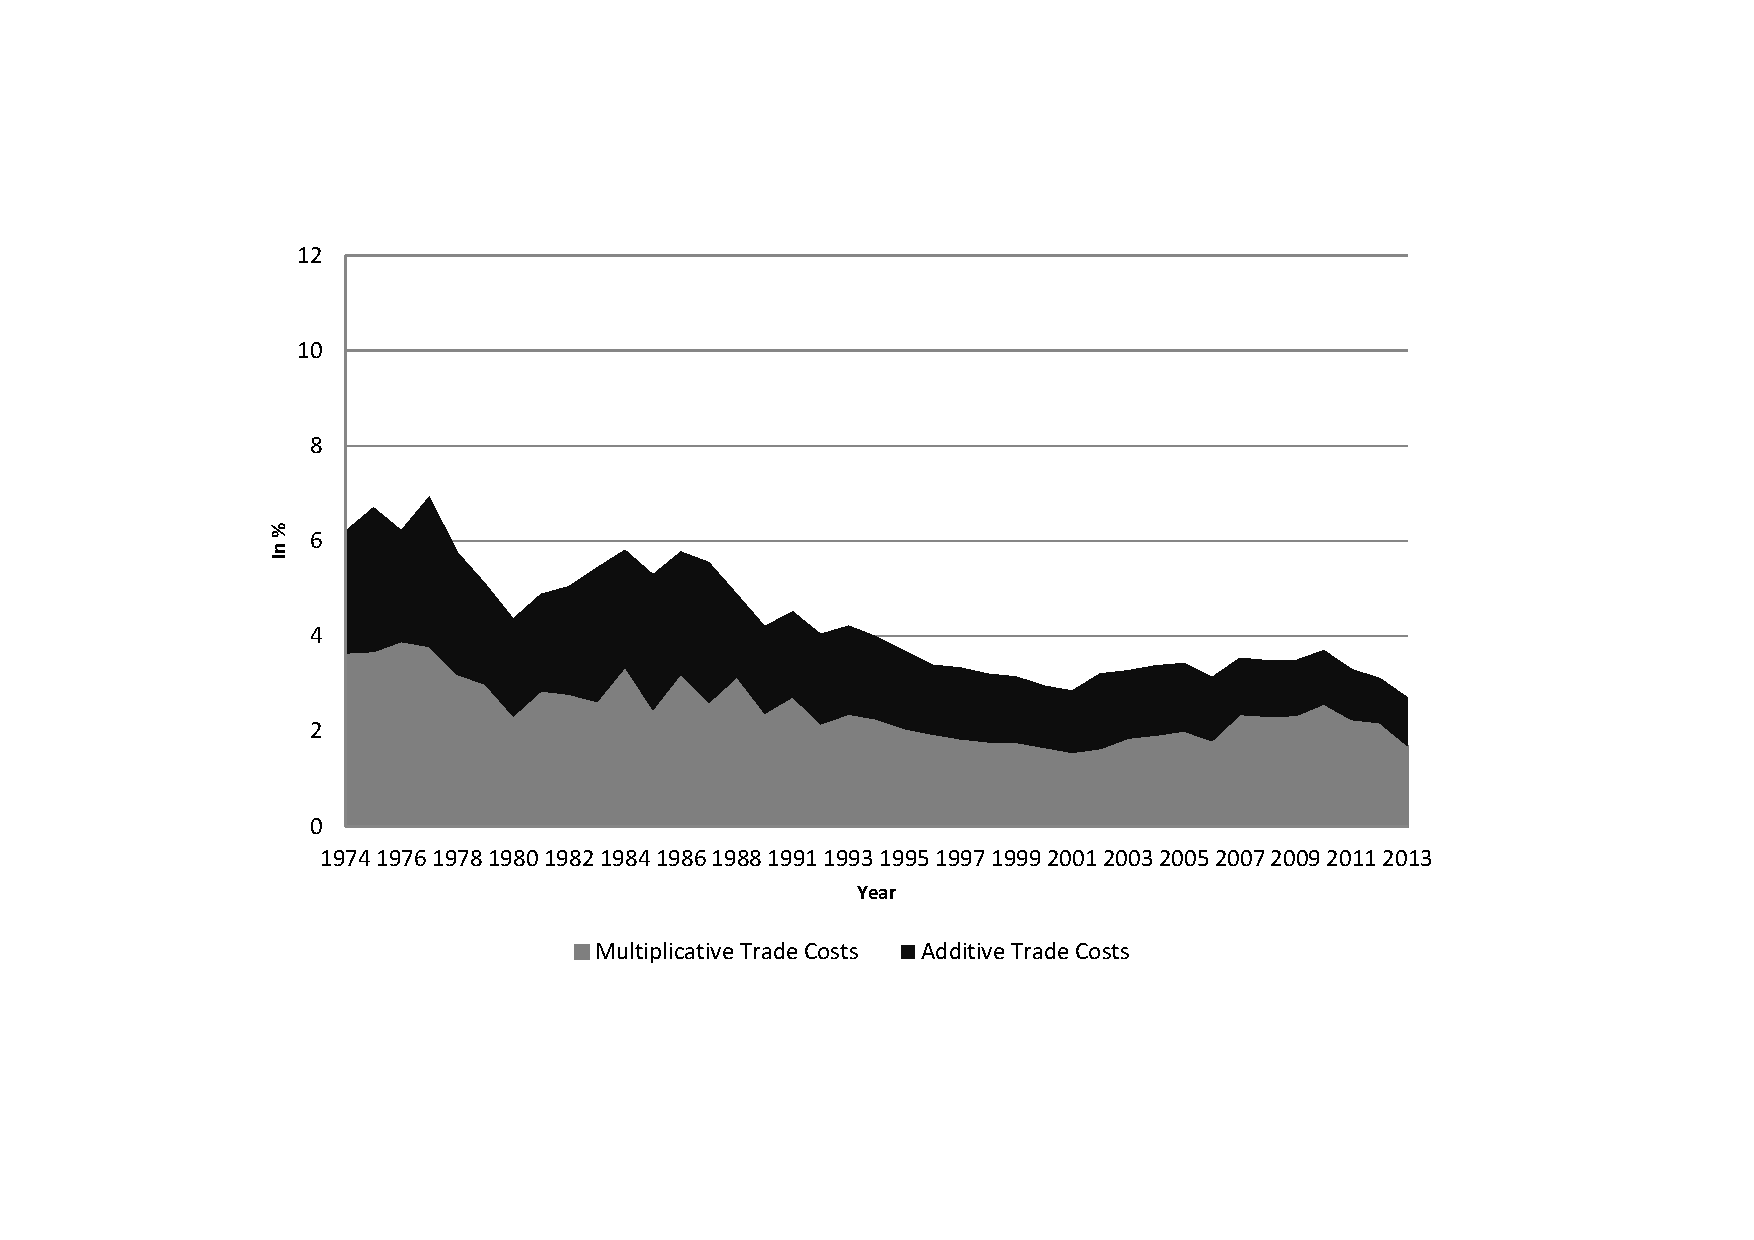
\includegraphics[width=5cm, height=4cm]{Fig2a_decompTC_air_3d.pdf}
& 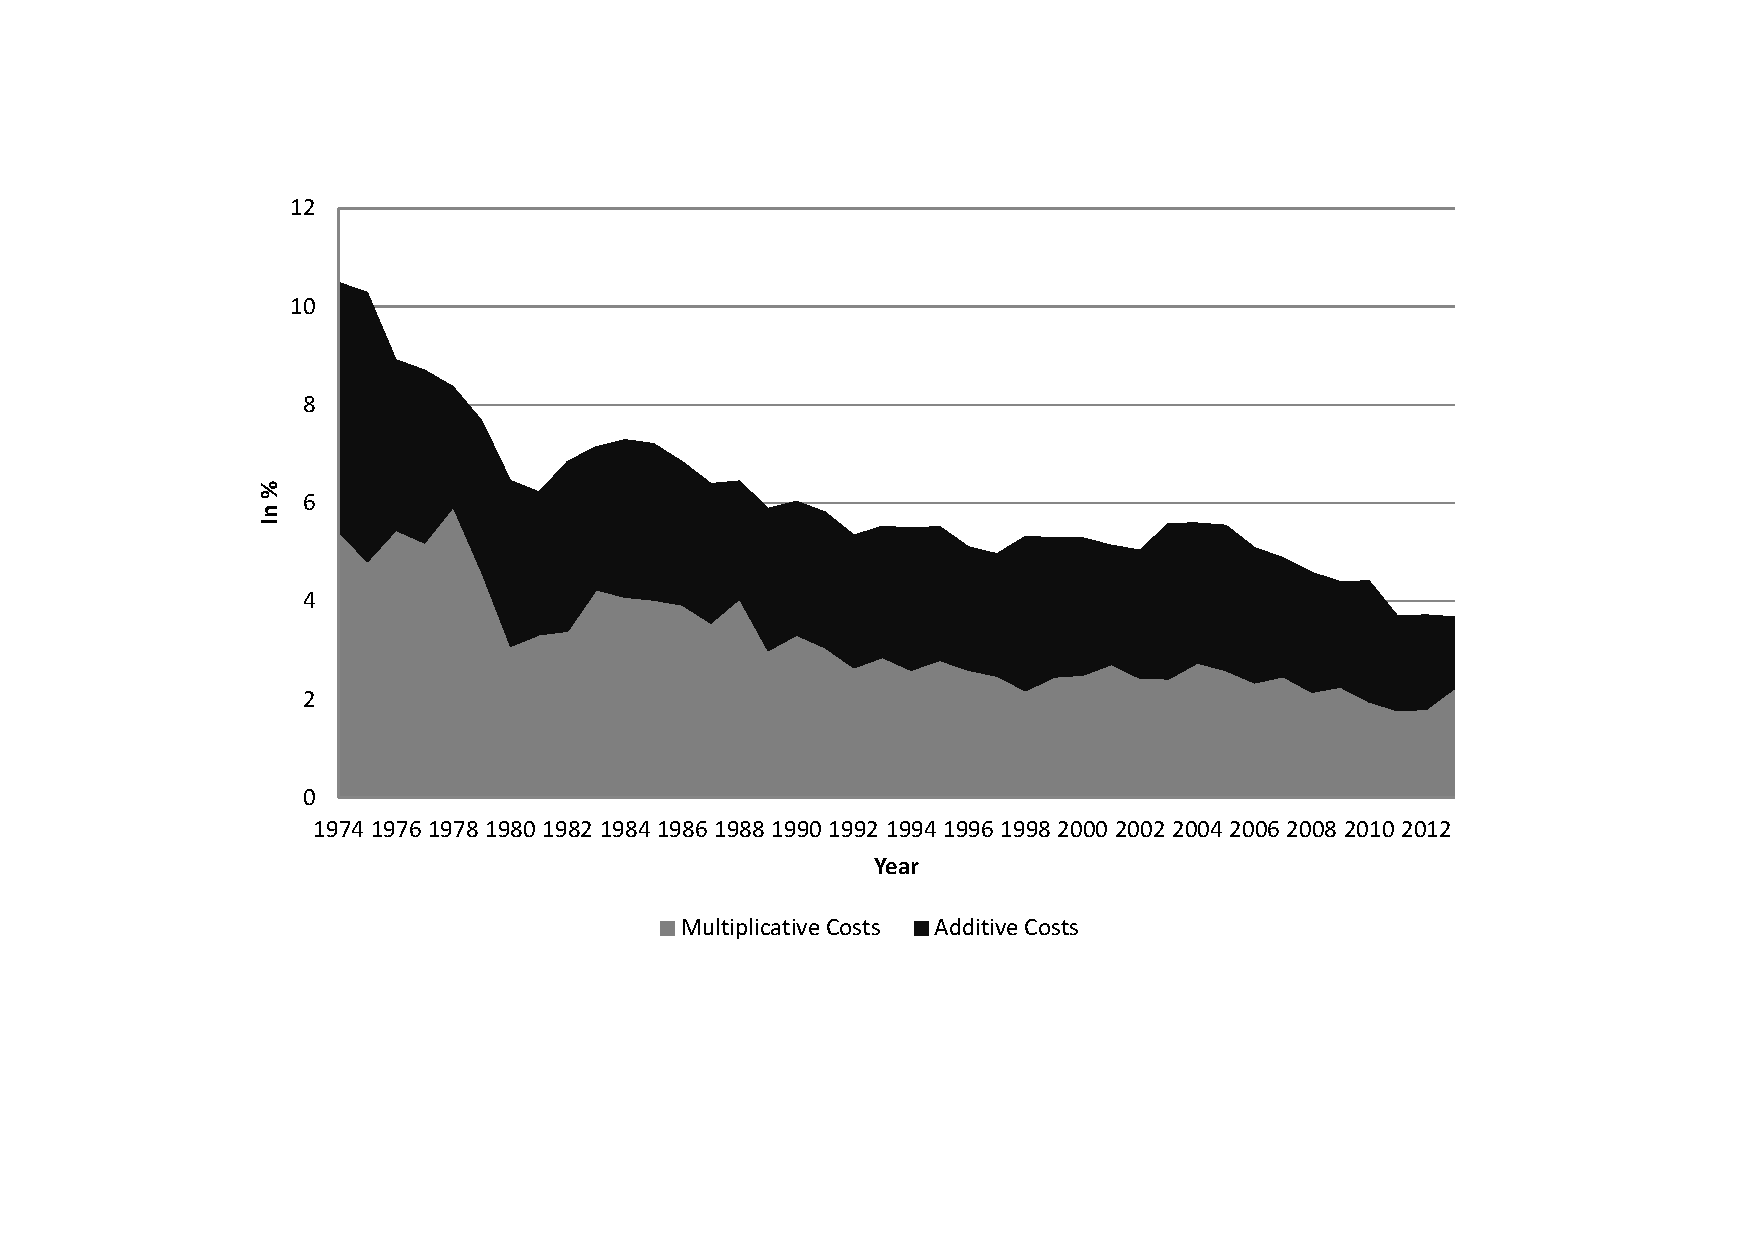
\includegraphics[width=5cm,height=4cm]{Fig2b_decompTC_vessel_3d.pdf} \\
\end{tabular}\end{center}
\end{figure}
\begin{itemize}
\item[-] Lower overall transport costs in Air than in Vessel \vspace{0.1cm}
\item[-] Downward trend for both modes since 1974 \vspace{0.1cm}
%\item[-] Slighlty ore pronounced in ocean shipping \vspace{0.1cm}
\begin{itemize}
\item[$\ast$] A 50\% decrease in Air, a 60\% decrease in Vessel over the period
\end{itemize}
\end{itemize}
\end{itemize}
\end{frame}


\begin{frame} [label = slide_compeffects_strategy]
\frametitle{Time trends in transport costs \& composition effects }
\begin{itemize}
\item Does it mean a decrease in transport costs \textit{per se}? Not necessarily \vspace{0.2cm}
\item The change in overall transport costs over time: \vspace{0.1cm}
\begin{itemize}
\item[-] Depend on the evolution of per product- per partner costs, \vspace{0.1cm}
\item[-] But also on the composition of trade flows \vspace{0.1cm}
\begin{itemize}
\item[$\star$] Over time, import more goods that are cheaper to transport, and/or from countries with which it is cheaper to trade \vspace{0.1cm}
\end{itemize}
\end{itemize}
\item[$\Rightarrow$] Necessary to eliminate the composition effects of trade flows, to isolate the evolution of transport costs \textit{per se}   \vspace{0.1cm}
\item[$\Rightarrow$] What we do, in accordance with Hummels (2007) \vspace{0.1cm}
\item Some insights on our methodology \hyperlink{app_compeffects_strategy}{\beamergotobutton{More details}} \hyperlink{app_compeffects_Hummels}{\beamergotobutton{Comparison with Hummels (2007)}} \vspace{0.1cm}
\begin{itemize}
\item[-] Start with estimates of additive/multiplicative transport costs  \vspace{0.1cm}
\item[-] Extract the ``pure'' TC component by the mean of a time fixed-effect \vspace{0.1cm}
%\item[-] For both the additive \& the multiplicative TC components \vspace{0.1cm}
\item[-] Build a unified measure of ``total'' transport costs (agglomerate the two components), also both fitted and unfitted
\end{itemize}
\end{itemize}
\end{frame}

\begin{frame}[label = slide_compeffects_figure]
\frametitle{Time trends in transport costs: Results}
\begin{itemize}
\item Transport costs over time (with and without composition effects)
\end{itemize}

\begin{figure}[htbp]
%\caption{Transport costs (with and without composition effects)}
%\label{fig:totalTC_compeffects_excl}
\begin{center}
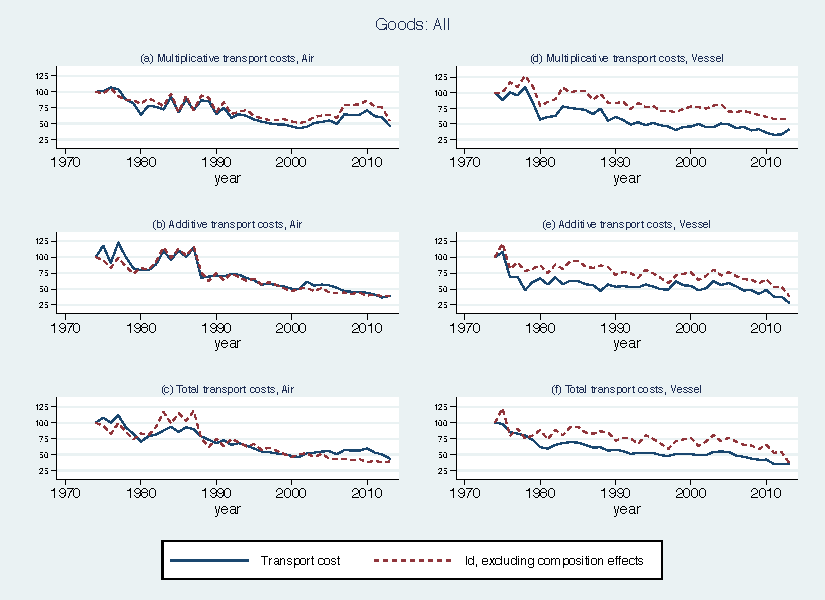
\includegraphics[height=7cm]
{graph_composition_all.pdf}
\end{center}
\end{figure}
\hyperlink{slide_compeffects_results}{\beamergotobutton{Back to slide}}
\end{frame}


\begin{frame}
\frametitle{Time trends in transport costs: Comments}
\begin{itemize}
\item A strong reduction of transport costs over the period (1974-2013) \vspace{0.1cm}
\begin{itemize}
\footnotesize
%\item[-] By 50\% in Air and 60\% in Ocean transport \vspace{0.1cm}
\item[-] Consistent with the literature, see Lafourcade \& Thisse (2011) \vspace{0.1cm}
\item[-] Roughly same order of magnitude for both the ad-valorem and the additive component  \vspace{0.1cm}
\normalsize
\end{itemize}
\item \textbf{Trade composition effects: A minor role in accounting for the time trend of TC}\vspace{0.1cm}
\begin{itemize}
\footnotesize
\item[-] Not much evidence of a difference between the ``raw'' and the ``pure'' TC components \vspace{0.1cm}
\normalsize
\end{itemize}
\item In Air transport \vspace{0.1cm}
\begin{itemize}
\footnotesize
\item[-] The 50\% decrease is mainly attributable to the reduction of ``pure'' transport costs, for both components  \vspace{0.1cm}
\end{itemize}
\normalsize
\item Composition effects (slightly) more pronounced in maritime transport \vspace{0.1cm}
\begin{itemize}
\footnotesize
\item[-] The 60\% decrease is roughly 50\% decrease of ``pure'' TC, 10\% decrease from composition effects \vspace{0.1cm}
\item[-] But for the multiplicative component only \vspace{0.1cm}
\end{itemize}
\normalsize
\end{itemize}
\end{frame}


\begin{frame}[label = slide_compeffects_results]
\frametitle{Time trends in transport costs: The role of additive costs}
\begin{itemize}
\item A result in sharp contrast with Hummels (2007) \vspace{0.1cm}
\begin{itemize}
\item[-] According to whom pure transport costs have decreased much more than the unfitted ones (over 1974-2004) \vspace{0.1cm}
\item[-] Suggesting an important role to trade composition effects  \vspace{0.1cm}
\end{itemize}
\item Not the case here. \vspace{0.1cm}
\item[$\Rightarrow$] \textbf{Where does the difference come from?} \vspace{0.1cm}
\item \textbf{From the treatment of the additive component of transport costs} \vspace{0.1cm}
\begin{itemize}
\item[-] Assuming (as we do, $\neq$ Hummels (2007)) a varying share of the additive component over time, product and country partner is key \vspace{0.1cm}
%\item[-] Strong impact in the decomposition of the time trend of transport costs, between composition effects and ``pure'' transport costs changes \vspace{0.1cm}
\item[-] What if we relax this assumption?
\end{itemize}\vspace{0.1cm}
\end{itemize}

\end{frame}


\begin{frame}
%\frametitle{Time trend of transport costs \& the modeling of the additive component}
\begin{itemize}
\item Assuming (as Hummels, 2007) a constant share of the additive component over time/country partner/product \vspace{0.1cm}
\item[$\Rightarrow$] Transport cost changes decompose as:
\begin{figure}[htbp]
%\caption{Transport costs (with and without composition effects)}
%\label{fig:totalTC_compeffects_excl}
\begin{center}
\begin{tabular}{cc}
{\scriptsize (a) Air } & {\scriptsize (b) Vessel}\\
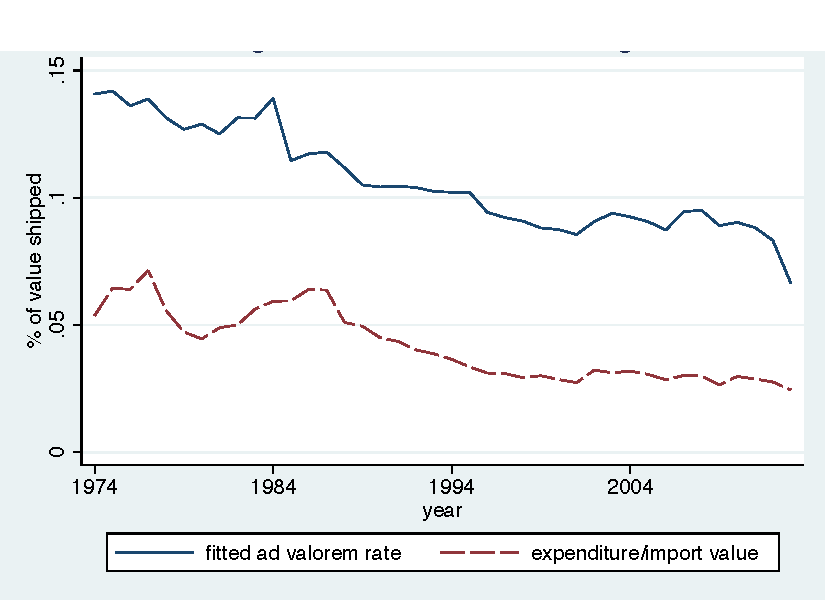
\includegraphics[width=5cm, height=4cm]{figure5_comme_hummels_air.pdf}
& 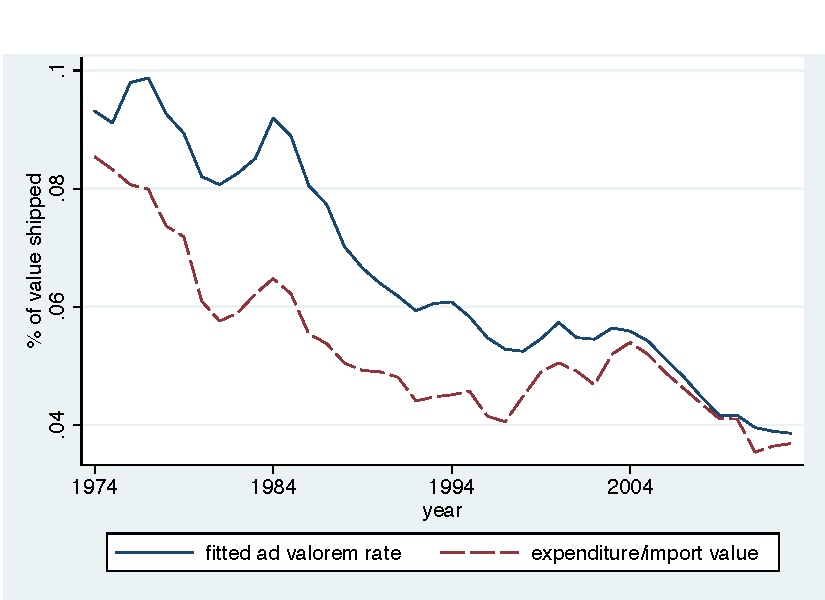
\includegraphics[width=5cm,height=4cm]{figure6_comme_hummels_ocean.pdf} \\
\end{tabular}
\end{center}
\end{figure}
\item[$\Rightarrow$] Suggest a much more important role to trade composition effects...  \vspace{0.1cm}
\item Than they actually do, see \hyperlink{slide_compeffects_figure}{\beamergotobutton{Figure 2}} \vspace{0.1cm}

\item[$\Rightarrow$] The (appropriate) modeling of additive costs, of key importance in understanding the time trends of international transport costs
\end{itemize}
\end{frame}


\begin{frame}
\frametitle{Conclusion: Main findings}
\textbf{Our paper: Empirical evidence about the role of the additive component in international transport costs} \vspace{0.1cm}
\begin{itemize}
\item Provide a quantitative evaluation of both the additive and the ad-valorem components \vspace{0.1cm}
\begin{itemize}
\item[-] Based on the US imports flows from 1974 to 2013 \vspace{0.1cm}
\item[-] Additive cost: amount to 2.8\% of the export price in ocean shipping, 1.8\% in air transport \vspace{0.1cm}
\item[-] Iceberg cost: 3.2\% and 2.5\% for air and ocean respectively \vspace{0.1cm}
\end{itemize}
\item The importance of taking into account additive transport costs \vspace{0.1cm}
\begin{itemize}
\item[-] Additive costs are sizeable quantitatively \vspace{0.1cm}
\item[-] A better fit of the model when they are taken into account    \vspace{0.1cm}
\item[-] A key role in the understanding of the time trend of transport costs
\end{itemize}

\end{itemize}

\end{frame}

\begin{frame}
\frametitle{Conclusion : What to do next?}

\textbf{Two main possible extensions}
\begin{itemize}
\item On the empirical side: Go deeper in the structural determinants of transport costs\vspace{0.1cm}
\begin{itemize}
\item[-] Identify the respective roles of handling costs, insurance and freight costs at the root of the import-export prices gap \vspace{0.2cm}
\end{itemize}
\item On the theoretical side: Use our results to explore the role of additive costs  \vspace{0.1cm}
\begin{itemize}
\item[-] In shaping international trade flows (trade theory) \vspace{0.1cm}
\item[-] In affecting the international transmission of business cycles (business cycle theory)
\end{itemize}
\end{itemize}
\end{frame}


\beginbackup



\appendix


\begin{frame}
\large
\center
\textsc{Appendix}
\normalsize
\end{frame}


\begin{frame}[label = app_empirical_strategy]
\frametitle{More on the empirical specification }
\textbf{The estimation strategy}
\begin{itemize}
\item Two assumptions (as in Irrarazabal et al., 2015) \vspace{0.1cm}
\begin{itemize}
\item[-] Both iceberg and additive costs are separable between the origin country $i$ and the product $k$ dimensions \vspace{0.1cm}
\item[-] Separability in a multiplicative manner for ad-valorem costs and additive manner for per-kg costs \vspace{0.1cm}
\end{itemize}
\footnotesize
\begin{eqnarray*}
\tau_{ik} = \tau_i \times \tau_k &\text{and}& t_{ik} = t_i + t_k
\end{eqnarray*}
\normalsize
\item Additional assumption: All products in a 3-digit sector ($s$) share the same structure of costs \vspace{0.1cm}
\item[$\Leftrightarrow$] Write $t_{is(k)}$ and $\tau_{is(k)}$ as:
\footnotesize
\begin{equation}
 \tau_{is(k)} = \tau_{i} \times \tau_{s(k)}, \qquad t_{is(k)} = t_{i} + t_{s(k)} \label{eq:specifTC}
 \end{equation}
 \normalsize
\end{itemize}
\end{frame}


\begin{frame}
\begin{itemize}
\item Given the constraint $\frac{p_{ik}}{\widetilde{p}_{ik}} >1$, the error term should be always positive and multiplicative \vspace{0.1cm}
\item[$\Rightarrow$] The equation of interest (\ref{eq:basis_equation}) becomes:
\footnotesize
$$\frac{p_{ik}}{\widetilde{p}_{ik}}-1 =\left(\tau_{i} \times \tau_{s(k)} -1+\frac{t_{i} + t_{s(k)}}{\widetilde{p}_{ik}} \right)\times \exp(\epsilon_{ik})$$
\normalsize
\item Taking logs, we finally estimate the following equation
\footnotesize
\begin{equation*}
\ln\left(\frac{p_{ik}}{\widetilde{p}_{ik}}-1 \right)= \ln \left(\tau_{i} \times \tau_{s(k)}+\frac{t_{i} + t_{s(k)}}{\widetilde{p}_{ik}}-1 \right) + \epsilon_{ik}
\end{equation*}
\normalsize
\begin{itemize}
\item[-] With $\epsilon_{ik}$ following a normal law centered on 0  \vspace{0.1cm}
\item[-] $\tau_i$, $\tau_{s(k)}$, $t_i$, $t_{s(k)}$ are the parameters (i.e. fixed effects) to be estimated
\end{itemize}
\item A non-linear equation (due to the additive costs)  \vspace{0.1cm}
\item[$\Rightarrow$] Estimation using non-linear squares 

\end{itemize}
\hyperlink{slide_empirical_strategy}{\beamergotobutton{Back to Slide}}
\end{frame}


\begin{frame}
\frametitle{More on the estimation method}
\begin{itemize}
\item Non-linear least square estimation method: Some insights \vspace{0.1cm}
\begin{itemize}
\item At the basis of the method: Approximate the model by a linear one and refine the parameters by successive iterations \vspace{0.1cm}
\item The criterion for convergence: That the sum of the squares of the residuals does not increase from one iteration to the next \vspace{0.2cm}
\end{itemize}
\item Eliminate potential influence of outliers: Exclude the 5 percent of the upper and lower tails of the distribution
\end{itemize}

\hyperlink{slide_empirical_strategy}{\beamergotobutton{Back to slide}}
\end{frame}

\begin{frame}[label=app_results_summary]
\frametitle{Decomposing transport costs: Summary \hyperlink{slide_results_summary}{\beamergotobutton{Back to slide}}}
\begin{table}[htbp]
  \centering
  \scriptsize{
  %\caption{Transport costs estimates: Summary \label{tab:summary_results}}
  \begin{center}
    \begin{tabular}{l|cc|cc}
      \hline \hline
    \multicolumn{5}{c}{Mean value over 1974-2013}   \\
    \# digit & \multicolumn{2}{c}{3 digits} & \multicolumn{2}{c}{4 digits ($^\ast$)} \\ \hline
    Mode  & Vessel & Air ($^{\ast \ast}$) & Vessel & Air \\ \hline
    \multicolumn{5}{l}{With only Ad-Valorem Trade Costs }  \\ \hline
    Mean  & 1.058 & 1.051 & 1.060 & 1.049 \\
    Median & 1.051 & 1.042 & 1.052 & 1.037 \\
    Std   & 0.032 & 0.042 & 0.036 & 0.045 \\
    Min. value & 1.003 & 1.001 & 1.003 & 1.000 \\
    Max. value & 1.304 & 1.685 & 1.408 & 2.051 \\ \hline
    \multicolumn{5}{l}{With Additive \& Ad-Valorem Trade Costs } \\ \hline
   \textit{Ad-valorem term} & & & & \\ \hline
    Mean  & 1.032 & 1.025 & 1.033 & 1.024 \\
    Median & 1.028 & 1.018 & 1.028 & 1.016 \\
    Std   & 0.023 & 0.023 & 0.025 & 0.026 \\
    Min. value & 1.001 & 1.000 & 1.000 & 1.000 \\
    Max. value & 1.227 & 1.474 & 1.264 & 1.537 \\ \hline
    \textit{Additive term }& & & &   \\ \hline
    Mean  & 0.029 & 0.018 & 0.028 & 0.019 \\
    Median & 0.019 & 0.007 & 0.017 & 0.008 \\
    Std   & 0.041 & 0.034 & 0.039 & 0.034 \\
    Min. value & 0.000 & 0.000 & 0.000 & 0.000 \\
    Max. value & 2.941 & 13.303 & 3.197 & 11.440 \\ \hline
        \# obs. & 29279 & 28207 & 29317 & 27680 \\
    \# origin country & 188 & 191 & 188 & 189 \\
    \# products & 230 & 211 & 666 & 567 \\  \hline \hline
  \end{tabular}
    \end{center}}
\parbox[l]{8cm}{\tiny{Notes: Statistics are obtained weighting each observation by its value. The additive term is expressed in fraction of fab price. ($^\ast$): Four 4-digit estimation: 0n selected years. ($^{\ast \ast}$): 1989 omitted in 3 digit estimation for air.}}
\end{table}%
\end{frame}


\begin{frame}[label=app_result1]
\frametitle{Size of transport costs: Comparison with the literature (1)}

\begin{itemize}
\item Size of overall transport costs \vspace{0.1cm}
\begin{itemize}
\item[-] Add $\simeq$ a 5\% margin over the export price \vspace{0.1cm}
\item[-] Lower than the 21\% markup taken from Anderson \& Van Wincoop (2004) (AWM), but  \vspace{0.1cm}
\begin{itemize}
\footnotesize{
\item[$\ast$] AVW decompose the 21\% markup in 9\% of time costs and 11\% in pure freight costs  \vspace{0.1cm}
\item[$\ast$] Their 11\% markup: A ``rough'' estimate, based on Hummels (2001) with 1994 data \vspace{0.1cm}
\item[$\ast$] Our data are only for the US, which presumably has lower trade costs } \vspace{0.1cm}
\end{itemize}
\end{itemize}
\item[$\Rightarrow$] Our work: A more precise and exhaustive estimation of international transport costs \vspace{0.1cm}
\end{itemize}
\hyperlink{slide_result1}{\beamergotobutton{Back to slide}}
\end{frame}


\begin{frame}
\frametitle{Size of transport costs: Comparison with the literature (2)}
\begin{itemize}
\item Size of additive transport costs: Comparison with Irarrazabal et al. (2015) \vspace{0.1cm}
\begin{itemize}
\item[-] Irarrazabal et al. (2015): Estimate the trade costs ratio $t/\tau$ = 14\% of the export price $\widetilde{p}$ \vspace{0.1cm}
\item[-] In 2004, our estimates lead to $t/\tau = 7.7\% \times \widetilde{p}$ (Air), $t/\tau = 1.5\%\times \widetilde{p}$ (Ocean) \vspace{0.1cm}
\item[$\Rightarrow$] Much lower !
\end{itemize}
\item But, our work: Estimate transport costs, not trade costs \vspace{0.1cm}
\begin{itemize}
\item[-] According to AVW, transport costs $\simeq$ 15\% of trade costs \vspace{0.1cm}
\item[-] Simple calculus thus implies that our estimates amount to 62\% (Air) and 53\% (Vessel) of Irarrazabal \& al.'s estimates \vspace{0.1cm}
\end{itemize}
\item[$\Rightarrow$] Additive transport costs represent between 1/2 and 2/3 of total additive trade costs
\end{itemize}
\hyperlink{slide_result1}{\beamergotobutton{Back to slide}}
\end{frame}


\begin{frame}[label=app_goodnessfit]
\frametitle{More on Result 2: Goodness of fit comparison}
\begin{itemize}
\item Air, 3 digit - level, selected years
\end{itemize}
\begin{table}[htbp]
  \centering
 % \caption{Air: Measures of Goodness-of-fit (3 digits)}
  \scriptsize{
\begin{center}
    \begin{tabular}{l|ccccc|c}
    \hline \hline
    Year  &1980  & 1990  & 2000  & 2010 & 2013 & Mean stat \\ \hline
    \multicolumn{7}{l}{\bf{$R^2$} }\\ \hline
    Term I only &  0.27  & 0.25  & 0.32  & 0.42 & 0.34 & 0.31 \\
    Terms A \& I &  0.65  & 0.63  & 0.64  & 0.51 & 0.46 & 0.60 \\ \hline
    \multicolumn{7}{l}{\textbf{SER}  }  \\ \hline
    Term I only &  0.86  & 0.81  & 0.84  & 0.86 & 0.92 & 0.85 \\
    Terms A \& I &  0.71  & 0.67  & 0.70  & 0.79 & 0.85 & 0.73 \\ \hline
   \multicolumn{7}{l}{\textbf{AIC criteria}}  \\ \hline
    Term I only &  41171.0 & 60715.6 & 87492.6 & 102297.6 & 88191.9 & 70498.1 \\
    Terms A \& I & 35738.4 & 52098.9 & 74954.9 & 95887.1 & 80873.7 & 62285.0 \\ \hline
    \multicolumn{7}{l}{\textbf{Log-likelihood}} \\ \hline
    Term I only &  -20253.5 & -29977.8 & -43341.3 & -50746.8 & -43692.9 & -34888.6 \\
    Terms A \& I &  -17263.2 & -25393.5 & -36788.4 & -47277.5 & -39751.9 & -30508.3 \\
    LL ratio &  5980.6 & 9168.7 & 13105.7 & 6938.6 & 7882.1 & 8760.69 \\
    nb of restrictions & 369   & 393   & 426   & 426 & 427 & 402 \\
    p-value & 0.00 & 0.00 & 0.00 & 0.00 & 0.00 & 0.00 \\
    \hline \hline
 \end{tabular}%
    \end{center}}
 % \label{tab:good_fit_air}%
% \parbox[l]{10cm}{\tiny{Notes: SER = Standard Error of regression; AIC = Akaike Information Criterion. $R^{2}$ between the log of predicted ratio and the log of the observed ratio. For the LL ratio test, the number of restrictions is equal to the number of parameters estimated, i.e., the number of partner countries plus the number of products. The mean statistics is calculated as the average value over all years. }}
\end{table}%
\hyperlink{slide_goodnessfit}{\beamergotobutton{Back to slide}}
\end{frame}

\begin{frame}
\frametitle{Goodness of fit comparison (cont')}
\begin{itemize}
\item Vessel, 3 digit - level, selected years
\end{itemize}
\begin{table}[htbp]
  \centering
  %\caption{Vessel: Measures of Goodness-of-fit (3 digits)}
    \scriptsize{
\begin{center}
\begin{tabular}{l|ccccc|c}
\hline \hline
Year  &  1980 & 1990 & 2000 & 2010  & 2013 & Mean stat \\ \hline
\multicolumn{7}{l}{\bf{$R^2$} }\\ \hline
Term I only &  0.415 & 0.456 & 0.401 & 0.350 & 0.339 & 0.39 \\
Terms A \& I &  0.575 & 0.590 & 0.571 & 0.491 & 0.462 & 0.56 \\ \hline
\multicolumn{7}{l}{\textbf{SER}  }  \\ \hline
    Term I only &  0.62 & 0.59 & 0.65 & 0.74  & 0.76 & 0.66 \\
    Terms A \& I &  0.53 & 0.51 & 0.55 & 0.66  & 0.68 & 0.57 \\ \hline
   \multicolumn{7}{l}{\textbf{AIC criteria}}  \\ \hline
    Term I only & 33010.3 & 51142.6 & 71365.9 & 84789.9 & 88191.9 & 57848.6 \\
    Terms A \& I &  28067.3 & 43664.7 & 60475.9 & 76161.3 & 80873.7 & 49682.3 \\ \hline
    \multicolumn{7}{l}{\textbf{Log-likelihood}} \\ \hline
    Term I only &  -16129.1 & -25169.3 & -35263.9 & -41998.9 & -43692.9 & -28534.3 \\
    Terms A \& I &  -13353.7 & -21171.4 & -29491.0 & -37418.7 & -39751.9 & -24151.3 \\
    LL ratio & 5550.96 & 7995.88 & 11545.98 & 9160.56 & 7882.15 & 8766.0 \\
    nb of restrictions  &  395 & 411 & 436 & 424   & 427 & 417 \\
    p-value & 0.00 & 0.00 & 0.00 & 0.00  & 0.00 & 0.00 \\
    \hline \hline
    \end{tabular}%
    \end{center}}
  \label{tab:good_fit_vessel}%
  \parbox[l]{10cm}{\tiny{Notes: SER = Standard Error of regression; AIC = Akaike Information Criterion. $R^{2}$ between the log of predicted ratio and the log of the observed ratio. For the LL ratio test, the number of restrictions is equal to the number of parameters estimated, i.e., the number of partner countries plus the number of products. The mean statistics calculated as the average value over all years. }}
\end{table}%
\hyperlink{slide_goodnessfit}{\beamergotobutton{Back to slide}}
\end{frame}


\begin{frame}
\frametitle{Goodness of fit: Comments}
\begin{itemize}
\item \textbf{Result 2}: Including the additive component improves the fit of the model, whatever the considered criterion or the transport mode \vspace{0.1cm}
\begin{itemize}
\footnotesize{
\item[-] On average over the period, the $R^2$ doubles for air transport, increases by 50\% for vessel (also on a yearly basis) \vspace{0.1cm}
}
\end{itemize}
\item A decrease in the quality of fit strongly after 2000, for both transport modes \vspace{0.1cm}
\item Contrasted results between air and ocean transports \vspace{0.1cm}
\begin{itemize}
\item[-] Ad-valorem costs have more explanative power in ocean shipping than in air transport \vspace{0.1cm}
\begin{itemize}
\item[$\ast$] On average, account for 39\% of the variance of the cif-fas ratio, vs 31\% in Air \vspace{0.1cm}
\end{itemize}
\item[-] But their explanatory power seems to have decreased over time \vspace{0.1cm}
\begin{itemize}
\item[$\ast$] For vessel: A roughly constant contribution of the additive component to the goodness of fit over time\vspace{0.1cm}
\end{itemize}
\item[$\neq$] For Air: The decreasing role of the explanatory power of the additive component over the recent years (consistent with Figure 1)\vspace{0.1cm}
\end{itemize}
\item[$\Rightarrow$] Go deeper in the analysis of the time-trends
\end{itemize}
\hyperlink{slide_goodnessfit}{\beamergotobutton{Back to slide}}
\end{frame}



\begin{frame}[label = app_compeffects_strategy]
\frametitle{Composition effects: Our strategy}
\begin{itemize}
\item Start with our estimates of add. \& adv. transport costs (TC) 
\begin{itemize}
\footnotesize
\item[-] That vary over time ($t$)/product ($k$) /origin country ($i$) (by transport mode): $\widehat{\tau}_{ikt}, \widehat{t}_{ikt}$ \vspace{0.1cm}
\end{itemize}
\item[$\Rightarrow$] Decompose the estimated TC component in three parts:  \vspace{0.1cm}
\begin{itemize}
\footnotesize
\item[-] Country dimension (Term (a)), product dimension (Term (b)) and the ``pure TC time trend'' (Term (c)).  \vspace{0.1cm}
%\item[-] Equations (\ref{eq:compeffects_mult}) and (\ref{eq:compeffects_add}): Preserve our specification of the ad-valorem and the additive costs (Equation (\ref{eq:specifTC}))
%\item[-] Equation (\ref{eq:compeffects_mult}) estimated using OLS, Equation (\ref{eq:compeffects_add}) using non-linear least squares (by transport mode)
\end{itemize}
\item For the ad-valorem component, we estimate the following equation:
\footnotesize
\begin{eqnarray}
\ln(\widehat{\tau}_{ikt})&=&\delta +\underbrace{\sum_{i \neq \text{ARG}}\alpha_i.\mathbb{1}_i}_{(a)} + \underbrace{\sum_{s(k)\neq \text{011}}\beta_{s(k)}.\mathbb{1}_{s(k)}}_{(b)} + \underbrace{\sum_{t \neq 1974}\gamma_t.\mathbb{1}_t}_{(c)}+\epsilon_{ikt} \label{eq:compeffects_mult}
\end{eqnarray}
\normalsize
\item For the additive component:
\footnotesize
\begin{eqnarray}
\ln(\widehat{t}_{ikt})&=&\ln\left( \delta + \underbrace{\sum_{i \neq \text{ARG}}  \alpha_i.\mathbb{1}_i}_{(a)}+\underbrace{\sum_{s(k)}\beta_{s(k)}.\mathbb{1}_{s(k)}}_{(b)}\right) + \underbrace{\sum_{t \neq 1974}\gamma_t.\mathbb{1}_t}_{(c)}+\epsilon_{ikt} \label{eq:compeffects_add}
\end{eqnarray}
\normalsize
\begin{itemize}
\item[-] With $\mathbb{1}_i$, $\mathbb{1}_{s(k)}$ and $\mathbb{1}_{t}$ country-, sector- and time- fixed effects \vspace{0.1cm}
\end{itemize}

\end{itemize}
\end{frame}


\begin{frame}
\begin{itemize}
\item Isolate the change in the time dimension of each TC component \vspace{0.1cm}
\begin{itemize}
\item[-] From the ad-valorem component estimation (Equation (\ref{eq:compeffects_mult})), build the variable $\Gamma_t$ ($\forall~t \geq 1974$):
\footnotesize
\begin{equation*}
 \Gamma^{adv}_t= \frac {\bar{\tau}_{1974}.\exp(\gamma_t)-1} {\bar{\tau}_{1974}-1}
\end{equation*}
\normalsize
\begin{itemize}
\item[$\ast$] with $\bar{\tau}_{1974} = \exp(\delta+\sum_i \alpha_i + \sum_k \beta_k$) the mean TC in 1974
\end{itemize}
\item[-] For the additive cost, build the variable ($\forall~t > 1974$)
\footnotesize
$$\Gamma^{add}_t = 100 \exp(\gamma_t)$$
\normalsize
\end{itemize}
\item The $\Gamma^{add}_t$ and $\Gamma^{adv}_t$ series:
\begin{itemize}
\item[-] How TC components have changed over time if we stick the composition of trade flows by product/ country partner to the one observed in 1974  \vspace{0.1cm}
\item[-] Interpretation in percentage changes, with an initial value of 100 for $t=1974$    \vspace{0.1cm}
\item[-] As indices, measures easily comparable
\end{itemize}
\end{itemize}

\end{frame}


\begin{frame}
\begin{itemize}
\item Rebuild a measure of ``total'' transport costs  \vspace{0.1cm}
\begin{itemize}
\item[-] As the sum of the two components (additive and ad-valorem) \vspace{0.1cm}
\item[-] On both the ``raw'' (unfitted) measures and the ``pure'' (fitted) measures \vspace{0.1cm}
\end{itemize}
\item For the unfitted measure, build (by transport mode)
\footnotesize
$$\widehat{tc}^{raw}_t= \widehat{\tau}^{adv}_t -1 + \widehat{t}_t$$
\normalsize
\begin{itemize}
\item[-] with $\widehat{\tau}^{adv}_t$ and $\widehat{t}_t$ estimated by year (see before) \vspace{0.1cm}
\item[-] From this, we build:
\footnotesize
$$\Gamma^{tc, raw}_t = 100\frac{\widehat{tc}^{raw}_t -1 }{\widehat{tc}^{raw}_{1974}-1}$$
\normalsize
\end{itemize}
\item For the fitted measure, start directly from the two indices just obtained, $\Gamma^{add}_t$ and $\Gamma_{t}^{adv}$:
\footnotesize
$$\Gamma^{tc, pure}_t = \omega_{x}\Gamma^{add}_t +(1-\omega_{x})\Gamma^{adv}_t $$
\normalsize
\begin{itemize}
\item[-] With $x={air, ~vessel}$ and $\omega_x$ the relative weight of the additive TC component in total cost in 1974 \vspace{0.1cm}
\item[-] Precisely, $\omega_{air}= 0.423$ and $\omega_{vessel}= 0.482$
\end{itemize}
\end{itemize}
\hyperlink{slide_compeffects_strategy}{\beamergotobutton{Back to slide}}
\end{frame}



\begin{frame}[label = app_compeffects_Hummels]
\frametitle{Composition effects: Comparing with Hummels (2007) (1)}
Reformulating Hummels's (2007) method  \vspace{0.1cm}
\begin{itemize}
\item Start from the observed cif-fas price gap $TC_{ikt} = \frac{p_{ikt} - \widetilde{p}_{ikt}}{\widetilde{p}_{ikt}}$ (by transport mode) \vspace{0.1cm}
\item \textbf{The unfitted TC measure}, $TC_t$: Take the mean yearly value by weighting each flow by its (relative) total value \vspace{0.1cm}
\item To get the fitted TC measure, start from the regression \vspace{0.1cm}
\footnotesize
\begin{equation}
\ln TC_{ikt} = \delta+ \beta \ln \frac{1}{\widetilde{p}_{ikt}} + \sum_{i,k}\alpha_{ik}.\mathbb{1}_{ik}+ \sum_{t}\gamma_{t}.\mathbb{1}_{t} + \epsilon_{ikt}
\label{eq:hummels}\end{equation}
\normalsize
\item Take the predict of the regression $\rightarrow$ $\widehat{TC}_{ikt}$   \vspace{0.1cm}
\item \textbf{The fitted TC measure}, $\widehat{TC}_t$: The unweighed average in the product/origin country dimension   \vspace{0.1cm}
\item To be compared to the unfitted ad-valorem rate $TC_t$ (by transport mode)

\end{itemize}


\end{frame}


\begin{frame}
%\frametitle{Composition effects: Comparing with Hummels (2007) (cont')}
Five differences with our method  \vspace{0.1cm}
\footnotesize
\begin{enumerate}

\item Hummels (2007) obtains the fitted ad-valorem rate in one step (the LHS is the observed price gap) while we use a 2-step approach (extract the fitted TC from the \textit{estimated} unfitted ad-valorem rate) - but a slight difference \vspace{0.1cm}
\item Hummels (2007) does not purge its measure of the fitted ad-valorem rate by the country-sector fixed effect  - but only a scale effect \vspace{0.1cm}
\item We separate the country-product fixed effects in two components (country / product), due to the number of fixed effects to estimate in the non-linear setting - robustness analysis to this point (in progress) \vspace{0.1cm}
\item We differ in the weighting scheme to obtain the yearly value of the fitted TC measure.  \vspace{0.1cm}
\begin{itemize}
\footnotesize
\item[-] Hummels (2007): The unweighed average value over the $i,k$ dimension \vspace{0.1cm}
\item[$\neq$] We weight each flow by its relative value in total trade flows observed in 1974 \vspace{0.1cm}
\item[-] Not much of a difference provided the weighting scheme in value is constant over time \vspace{0.1cm}
\item[-] Robustness to the alternative weighting scheme (apply Hummels's (2007) method) in progress
\end{itemize}

\end{enumerate}
\normalsize

\end{frame}


\begin{frame}
\textcolor{blue}{5.} Last difference - the major one !
\begin{itemize}
\item Coming back to Hummels's (2007) equation (\ref{eq:hummels}), rewritten as:
\footnotesize
\begin{equation}
\ln TC_{ikt} \equiv \ln\left(\frac{p_{ikt}-\widetilde{p}_{ikt}}{\widetilde{p}_{ikt}}  \right) = \Delta_{ikt} - \beta \ln \widetilde{p}_{ikt} \label{eq:hummels2}
\end{equation}
\begin{itemize}
\item[-] with $\Delta_{ikt} \equiv \delta+ \sum_{i,k}\alpha_{ik}.\mathbb{1}_{ik}+ \sum_{t}\gamma_{t}.\mathbb{1}_{t} + \epsilon_{ikt}$
\end{itemize}
\normalsize
\item Encompasses the two extreme cases of only ad-valorem costs / only additive costs
\item Only multiplicative costs under $\beta=0$
\begin{itemize}
\item[-] In which case Equation (\ref{eq:hummels2}) rewrites as:
$$\ln\left(\frac{p_{ikt}-\widetilde{p}_{ikt}}{\widetilde{p}_{ikt}}  \right) = \Delta_{ikt} ~~\leftrightarrow~~ p_{ikt} = \underbrace{[\exp(\Delta_{ikt})+1]}_{\tau_{ikt}}\times \widetilde{p}_{ikt} $$
%\item[$\Rightarrow$] Only multiplicative costs
\end{itemize}
\item Only additive costs under $\beta=1$
\begin{itemize}
\item[-] In which case Equation (\ref{eq:hummels2}) rewrites as:
$$\ln\left(p_{ikt}-\widetilde{p}_{ikt}\right) = \Delta_{ikt} ~~\leftrightarrow~~ p_{ikt} = \widetilde{p}_{ikt} + \underbrace{[\exp(\Delta_{ikt})+1]}_{t_{ikt}}$$
%\item[$\Rightarrow$] Only additive costs
\end{itemize}
\end{itemize}

\end{frame}

\begin{frame}
\begin{itemize}
\item As noted by Hummels \& Skiba (2004), $0<\beta<1$ is the elasticity of freight costs to the export price \vspace{0.1cm}
\item Measures the relative weight of the additive component in international transport costs \vspace{0.1cm}
\begin{itemize}
\item[-] The higher $\beta$ close to 1, the larger the share of additive costs \vspace{0.1cm}
\end{itemize}
\item By estimating Equation (\ref{eq:hummels}) \textbf{with a constant $\beta$}, Hummels (2007) assumes a constant share of additive costs over time/country partner/product \vspace{0.1cm}
\item A key difference with our method \vspace{0.1cm}
\begin{itemize}
\item[-] Our strategy to obtain the transport costs measures explicitly allows for an additive component that varies in the 3 dimensions \vspace{0.1cm}
\end{itemize}
\item A key importance in the decomposition of time trends of transport costs (between the role of trade composition effects and the ``pure'' transport costs dimension)
\end{itemize}
\hyperlink{slide_compeffects_strategy}{\beamergotobutton{Back to main slide}}
\end{frame}




\end{document}
